To invoke the GUI, a designated button has to be pressed.
The default for this, although remappable, is the B button, which many controllers have.
When pressing the button once, they GUI will be attached to the backside of the users left hand.
By pressing the button once again, the GUI will be fixed in the current position.
This way, users can customize the GUIs location as they like without disturbing the workflow.
It also allows for better interaction with the virtual hands (Requirements \ref{req::N2}, \ref{req::N5}).
Another press of the button will hide the GUI.
\\ The GUI consists of the Restart, Case, Patient and Segment submenu.
To interact with the GUI, users use their virtual hands and simulate a real button press by virtually "pressing" their fingers on the GUI.
The GUI, acting as a wall, collides with the virtual hands, meaning the hands will not pass through the GUI.
This collision detection has been set up in such a way that the GUI can only collide with the virtual hands.
A slight haptic feedback in the form of the controller vibrating and visual feedback, i.e. toggling elements on and off, signals the user that a button has been pressed.
By pressing the Restart button, the user will be teleported back to the OT selection as described in Section \ref{sec::VirtualOperatingRoom}.
The first graphical interface which the user will see when pressing the button is the Case submenu (Figure \ref{fig::UIProjectCase}).
\begin{figure}[ht]
    \centering
    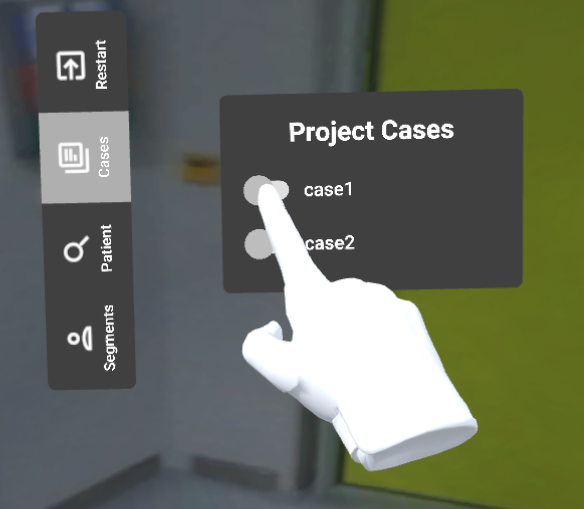
\includegraphics[width=200px]{images/implementation/user_interface/project_cases.png}
    \caption{\label{fig::UIProjectCase}GUI component for the selection of project cases.}
\end{figure}

This submenu shows all available project cases to the user.
The buttons for loading a case are created dynamically and depend on the number of project case JSON files found in the specified folder.
By pressing the button with the virtual hands, the project case will be loaded and the patient model and case information 
written down in the project case will be displayed from within the virtual OT.
The default position when a patient is loaded is hovering over the operating table in the OT.
On the left side of the GUI, the individual submenus can be selected.
Visualization tools can be selected via clicking on the Patient submenu, as depicted in Figure \ref{fig::UIPatientSegments}.
Here, tools which are the same for any project case can be used for visualization purposes.
Users have the option to scale the patient, look at the unprocessed patient for comparison and the ability to explode the 3D model to help with visualization.
Project cases can also be saved from this menu.

\begin{figure}[ht]
    \centering
    \begin{minipage}{.5\textwidth}
      \centering
      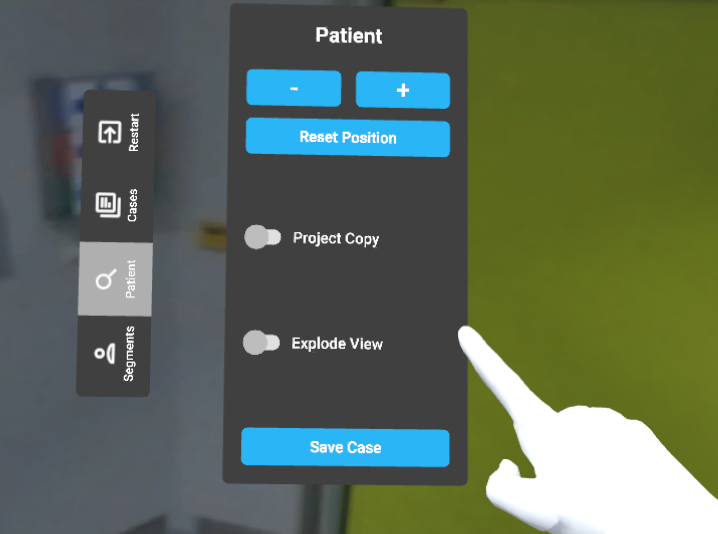
\includegraphics[width=0.99\linewidth]{images/implementation/user_interface/patient.png}
    \end{minipage}%
    \begin{minipage}{.5\textwidth}
      \centering
      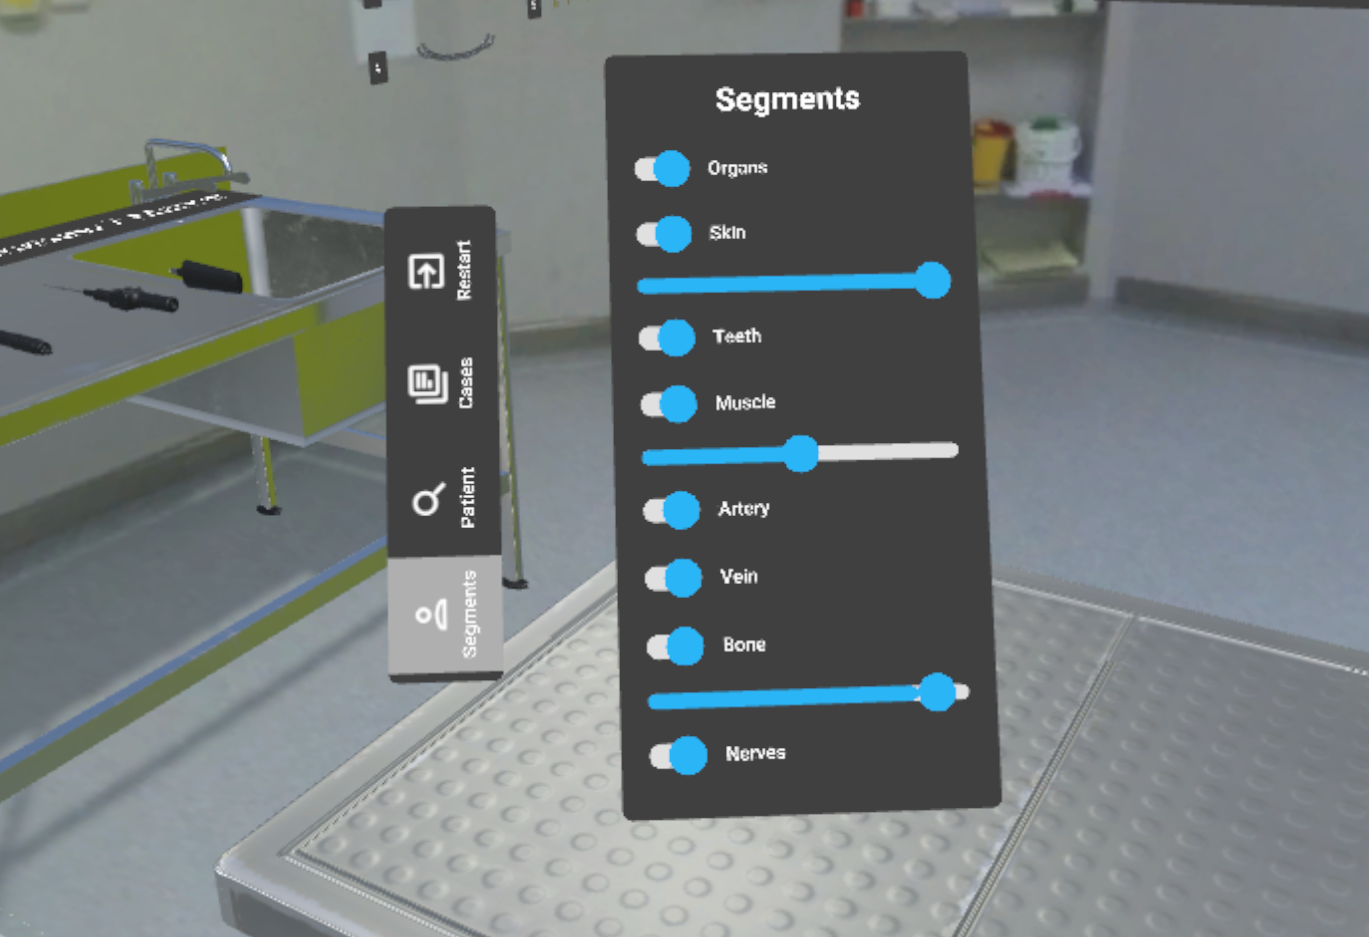
\includegraphics[width=0.99\linewidth]{images/implementation/user_interface/segments.png}
    \end{minipage}
    \caption{\label{fig::UIPatientSegments}Submenus for selecting different visualization tools provided by the system. The Patient submenu is consists of general visualization tool, while the segment submenu consists of patient-specific options for the segments.}
  \end{figure}